\documentclass{standalone}
\usepackage{pgfplots}
\pgfplotsset{soldot/.style={color=black,only marks,mark=*},
             holdot/.style={color=black,fill=white,only marks,mark=*},
             compat=1.12}
\begin{document}
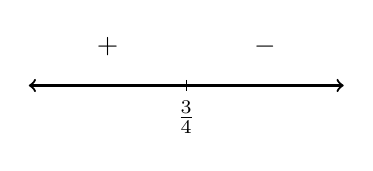
\begin{tikzpicture}
\draw[thick,<->] (-2,0) -- (2,0);
  \draw (0 cm,2pt) -- (0 cm,-2pt) node[anchor=north] {$\frac{3}{4}$};

 \draw (-1,.5) node {$+$};
 \draw (1,.5) node {$-$};

\end{tikzpicture}
\end{document}